\documentclass[11pt]{article}
\usepackage{amsmath, amssymb, amsthm}
\usepackage[retainorgcmds]{IEEEtrantools}

\usepackage[pdftex]{graphicx}
\usepackage{circuitikz}
\usepackage{tikz}
\usetikzlibrary{intersections}

\usepackage{fancyhdr}

%Format stuff
\pagestyle{fancy}
\headheight 35pt

%Header info
\chead{\Large \textbf{Electrical Systems}}
\lhead{}
\rhead{}

\begin{document}
\section{Components}
	\subsection{Capacitors}
		Capacitors are composed two metallic plates sandwiching some capcitating material (air, plastic, etc...). The plates acquire opposing charges of $Q$ and $-Q$ when charged.
		
		\begin{center}
		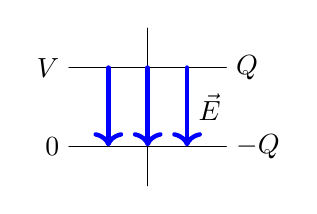
\begin{tikzpicture}
			[scale=1,line cap=round,
			%Styles
			axes/.style=,
			important line/.style={very thick},
			information text/.style={rounded corners,fill=red!10,inner sep=1ex},
			dot/.style={circle,inner sep=1pt,fill,label={#1},name=#1}			
			]
			
			%Colors
			\colorlet{anglecolor}{green!50!black}	%angle arcs/lines
			
			%The graphic
			\draw (1, .5) -- (1, 0);
			\draw node[left]{$V$} (0,0) -- (2, 0) node[right]{$Q$};
			\draw (0, -1) node[left]{$0$} (0, -1) -- (2, -1) node[right]{$-Q$};
			\draw (1, -1) -- (1, -1.5);
			
			\draw[blue,ultra thick,->] (.5, 0) -- (.5, -1);
			\draw[blue,ultra thick,->] (1, 0) -- (1, -1);
			\draw[blue,ultra thick,->] (1.5, 0) -- node[right,black]{$\vec{E}$} (1.5, -1);
		\end{tikzpicture}
		\end{center}
		
		The \textbf{capacitance} of a capacitor is a measure of how much charge it can hold relative to the potential difference between the two plates, and is measured in units Farads ($F$).
		\begin{equation}
			C = \frac{Q}{V}
		\end{equation}
		
		\subparagraph{Energy} A capacitor stores energy in the electric field between the plates. This can be expressed in terms of the \textbf{energy density}, $u$, and volume or the capacitance, charge, and potential difference.
		\begin{IEEEeqnarray}{rCl}
			U & = & \frac{1}{2}uV\\
			u & = & \epsilon_0 |\vec{E}|^2
		\end{IEEEeqnarray}
		\begin{equation}
			U = \frac{1}{2} QV = \frac{1}{2} CV^2 = \frac{Q^2}{2C}
		\end{equation}
	
	\subsection{Inductors}
		An inductor is a solenoid (coiled wire). Current induces a magnetic flux in the direction dictated by the right-hand-rule, creating a magnetic field. The \textbf{inductance} of an inductor measures its strength, and is in units of Henry ($H$).
		
		\begin{equation}
			L = \frac{\Phi_B}{I}
		\end{equation}
		
		\begin{equation}
			V = -L\frac{dI}{dt}
		\end{equation}
		
		Note that we define $I = -\dot{Q}$.
		
		\subparagraph{Energy} An inductor stores energy in the magnetic field generated by the changing current. This energy can be expressed in terms of the field strength and volume or inductance and current.
		\begin{equation}
			U_B = \frac{1}{2 \mu_0} |\vec{B}|^2 V
		\end{equation}
		\begin{equation}
			U_B = \frac{1}{2} LI^2
		\end{equation}
		
	\subsection{Resistors} 
		Resistors turn current into heat, serving as a current dampener in electrical systems. The \textbf{resistance} of a resistor is a measure of its strength, measured in units of Ohms ($\Omega$).
		\begin{equation}
			V = IR
		\end{equation}
		
\section{LC Circuits}
	LC circuits are the electrical analog to physical simple harmonic oscillators.
	\begin{center}
	\begin{circuitikz}
		\draw(0,0) to[C] (0, 2) -- (2, 2)
			to[L] (2, 0) -- (0, 0);
	\end{circuitikz}
	\end{center}
	
	By Kirchoff's rules,
	\begin{IEEEeqnarray}{rCl}
		V_C + V_L & = & 0\\
		\frac{Q}{C} - L\frac{dI}{dt} & = & 0\\
		\frac{Q}{C} + L\ddot{Q} & = & 0\\
		\ddot{Q} + \frac{1}{LC}Q & = & 0
	\end{IEEEeqnarray}
	
	If we define $\omega_0 = 1/LC$, then this is exactly the same as a SHO.
	\begin{equation}
		Q(t) = Q_0 e^{i(\omega t + \delta)}
	\end{equation}
	
\section{RLC Circuits}
	Undriven RLC circuits are the electical analog to dampened oscillators.
	
	\begin{center}
	\begin{circuitikz}
		\draw(0, 0) to[C] (0, 2) to[R] (2,2) to [L] (2, 0) -- (0, 0);
	\end{circuitikz}
	\end{center}
	
	\begin{IEEEeqnarray}{rCl}
		V_C + V_L + V_R & = & 0\\
		\frac{Q}{C} + R\dot{Q} + L\ddot{Q} & = & 0\\
		\ddot{Q} + \frac{R}{L}\dot{Q} + \frac{1}{LC}Q & = & 0
	\end{IEEEeqnarray}	
	
	Define $\gamma = R/L$ and this becomes the same thing as a dampened oscillator.
	\begin{equation}
		Q(t) = Q_0 e^{\gamma t / 2} e^{i(\omega_d t + \delta_d)}	
	\end{equation}		
	\begin{equation}
		\omega_d = \sqrt{\omega_0^2 - \frac{\gamma^2}{4}}
	\end{equation}
	
\section{Driven RLC Circuits}
	\begin{center}
	\begin{circuitikz}
		\draw(0, 0) to[C] (0, 2) to[R] (2,2) to[L] (2, 0) to[vsourcesin] (0, 0);
	\end{circuitikz}
	\end{center}
	
	\begin{equation}
		\ddot{Q} + \gamma\dot{Q} + \omega_0^2 Q = \frac{V_0}{L}e^{i\omega_s t}
	\end{equation}
	
	The steady-state solution is in the same form again.
	\begin{equation}
		Q(t) = Q_0 e^{i(\omega_s t + \delta)}
	\end{equation}
	\begin{equation}
		Q_0 = \frac{V_0/L}{\sqrt{(\omega_0^2 - \omega^2)^2 + (\omega\gamma)^2}}
	\end{equation}
	\begin{equation}
		\delta = -\tan^{-1}\left(\frac{\omega\gamma}{(\omega_0^2 - \omega^2)}\right)
	\end{equation}

%	\begin{center}
%	\begin{tikzpicture}
%		[scale=3,line cap=round,
%		%Styles
%		axes/.style=,
%		important line/.style={very thick},
%		information text/.style={rounded corners,fill=red!10,inner sep=1ex},
%		dot/.style={circle,inner sep=1pt,fill,label={#1},name=#1}			
%		]
%		
%		%Colors
%		\colorlet{anglecolor}{green!50!black}	%angle arcs/lines
%		
%		%The graphic
%	\end{tikzpicture}
%	\end{center}

%	\begin{figure}[htb]
%		\centering
%		\includegraphics[width=0.8\textwidth]{filename.eps}
%		\caption{Caption.}
%		\label{fig:figure}
%	\end{figure}

%		\def\enotesize{\normalsize}
%		\theendnotes
\end{document}